\documentclass{article}
\usepackage[utf8]{vietnam}
\usepackage[backend=biber,natbib=true,style=alphabetic,maxbibnames=50]{biblatex}
\addbibresource{references.bib}
\usepackage{tocloft}
\renewcommand{\cftsecleader}{\cftdotfill{\cftdotsep}}
\usepackage[colorlinks=true,linkcolor=blue,urlcolor=red,citecolor=magenta]{hyperref}
\usepackage{amsmath,amssymb,amsthm,enumitem,eurosym,fancyvrb,float,graphicx,mathtools,tikz,tabularx,booktabs}
\usetikzlibrary{angles,arrows.meta,calc,intersections,matrix,patterns,quotes,shadings}
\allowdisplaybreaks

\newtheorem{example}{Example}
\newtheorem{problem}{Problem}
\newtheorem{question}{Question}
\newtheorem{remark}{Remark}

\newtheorem{vidu}{Ví dụ}
\newtheorem{baitoan}{Bài toán}
\newtheorem{cauhoi}{Câu hỏi}
\newtheorem{nhanxet}{Nhận xét}

\usepackage[margin=1.61803398875cm]{geometry} % Golden ratio margin

\def\labelitemii{$\circ$}
\DeclareRobustCommand{\divby}{%
	\mathrel{\vbox{\baselineskip.65ex\lineskiplimit0pt\hbox{.}\hbox{.}\hbox{.}}}%
}
\setlist[itemize]{leftmargin=*}
\setlist[enumerate]{leftmargin=*}

\title{Some Decision Problems: A Personal Perspective\\ Vài Bài Toán Quyết Định: 1 Góc Nhìn Cá Nhân}
\author{Nguyễn Quản Bá Hồng\footnote{A scientist-\textit{\&} creative artist wannabe.\\E-mail: \sf nguyenquanbahong@gmail.com. Website: \url{https://nqbh.github.io/}. GitHub: \url{https://github.com/NQBH}.}}
\date{\today}

\begin{document}
\maketitle

\begin{abstract}
	In this work, I formalize several decision problems across academic, psychological, and philosophical domains. By applying computational and game-theoretic heuristics to both cognitive optimization tasks and adversarial interpersonal dynamics, this essay offers structured, pragmatic frameworks for navigating complex uncertainty.
	
	Trong tác phẩm này, tôi hình thức hóa 1 số bài toán quyết định vắt ngang qua các miền học thuật, tâm lý học, \& triết học. Thông qua việc áp dụng các phương pháp heuristic mang tính tính toán \& lý thuyết trò chơi vào cả những tác vụ tối ưu hóa nhận thức lẫn các động lực tương tác cá nhân đầy thù địch, bài tiểu luận này cung cấp những bộ khung thực chứng, có cấu trúc nhằm lèo lái qua những bất định phức tạp.
	
	This manuscript is part of the ongoing series \textit{Some Topics in Advanced STEM \& Beyond}:
	
	Bản thảo này là 1 phần của chuỗi bài viết đang tiếp diễn \textit{Một số Chủ đề trong STEM Nâng cao \& Hơn thế nữa}:
	\begin{center}
		\url{https://nqbh.github.io/advanced_STEM/}
	\end{center}
\end{abstract}

\tableofcontents
\clearpage

%------------------------------------------------------------------------------%
\section{Preface}
%------------------------------------------------------------------------------%

\textit{There are billions of people out there who can always make much better decisions than me for every single problem. Then why did I decide to write this text?} The answer is straightforward: Because decision-making does not come naturally to me, I have been forced to deconstruct and learn it from first principles. \textit{With this reason, will you read this text?}

\textit{Có hàng tỷ người ngoài kia luôn có thể đưa ra những quyết định tuyệt vời hơn tôi rất nhiều đối với từng vấn đề đơn lẻ. Vậy thì cớ sao tôi lại quyết định viết nên văn bản này?} Câu trả lời thực sự trực diện: Bởi lẽ việc ra quyết định vốn dĩ chẳng phải là 1 thiên bẩm của tôi, nên tôi đã buộc phải giải cấu trúc \& học hỏi nó từ những nguyên lý đầu tiên (first principles). \textit{Với lý do này, bạn sẽ đọc văn bản này chứ?}

\subsection{Disclaimer}
\begin{itemize}
	\item All scenarios and analytical frameworks presented herein represent personal theoretical reflections.
	
	\item \textit{Bản dịch:} Mọi kịch bản \& bộ khung phân tích được trình bày trong đây đều đại diện cho những suy ngẫm lý thuyết mang tính cá nhân.
\end{itemize}

\subsection{Goals}
\begin{itemize}
	\item Uncover structural and aesthetic beauty across interdisciplinary decision models.
	
	\item \textit{Bản dịch:} Khai phá vẻ đẹp cấu trúc \& thẩm mỹ xuyên suốt các mô hình quyết định liên ngành.
	
	\item Provide clear, actionable decision heuristics for navigating complex academic, professional, and psychological dilemmas.
	
	\item \textit{Bản dịch:} Cung cấp các phương pháp heuristic ra quyết định rõ ràng, có khả năng thực thi nhằm lèo lái qua những tình thế tiến thoái lưỡng nan phức tạp trong học thuật, nghề nghiệp, \& tâm lý học.
\end{itemize}

%------------------------------------------------------------------------------%
\section{Some Academic Decision Problems}
%------------------------------------------------------------------------------%

\subsection{Frog--Eagle Dilemma}

In his celebrated 2009 address, \textit{Birds and Frogs} \cite{dyson2009birds}, the physicist Freeman Dyson elegantly taxonomized the cognitive architectures of mathematicians---and by extension, all problem-solvers---into two fundamental archetypes. \textit{Birds}, Dyson observed, soar through the aether, surveying sweeping conceptual vistas to forge unifying theories that bridge disparate intellectual landscapes. \textit{Frogs}, conversely, dwell in the terrestrial mud, their gaze anchored to the exquisite intricacies of their immediate surroundings; they dismantle problems sequentially, discovering profound beauty in granular, structural depth. The edifice of human knowledge relies upon the symbiosis of both: it demands the breathtaking, Cartesian synthesis of the bird and the meticulous, Baconian empiricism of the frog.

Trong bài diễn văn nổi tiếng năm 2009, \textit{Birds and Frogs} \cite{dyson2009birds}, nhà vật lý Freeman Dyson đã phân loại 1 cách thanh tao các kiến trúc nhận thức của giới toán học---và mở rộng ra là của tất cả những người giải quyết vấn đề---thành hai nguyên mẫu nền tảng. \textit{Những chú chim}, Dyson quan sát thấy, chao lượn giữa không trung, khảo sát những tầm nhìn khái niệm bao quát để kiến tạo nên những lý thuyết thống nhất làm nhịp cầu nối liền các cảnh quan tri thức biệt lập. Ngược lại, \textit{những chú ếch} ngụ cư dưới bùn lầy mặt đất, ánh nhìn của chúng cắm chặt vào những sự phức tạp tinh xảo của môi trường xung quanh ngay lập tức; chúng tháo dỡ các vấn đề 1 cách tuần tự, khám phá ra vẻ đẹp sâu thẳm trong chiều sâu cấu trúc \& dạng hạt. Tòa tháp tri thức của nhân loại dựa dẫm vào sự cộng sinh của cả hai: nó đòi hỏi sự tổng hợp Descartes ngoạn mục của loài chim \& chủ nghĩa kinh nghiệm Bacon tỉ mỉ của loài ếch.

Building upon Dyson's framework, we elevate the avian archetype to that of the \textit{eagle}---an apex visionary wielding not merely a macroscopic vantage, but a commanding, dictatorial clarity over the operational theater.\footnote{Original thought expressed in Vietnamese: \textit{``Từng nghe câu chuyện về đại bàng \& ếch chưa? Nôm na: Đại bàng luôn bay cao, có tầm nhìn xa trông rộng, nên có thể bao quát được mọi thứ, giống kiểu của thiếu niên thiên tài trong Ao Ashi vậy---có tầm nhìn cực rộng nên có thể bao quát được cả sân bóng, phù hợp với lối chơi kiến tạo, điều khiển thế trận. Còn ếch thì dưới mặt đất, có khi ngồi sâu dưới đáy giếng, không nhìn thấy bức tranh toàn cảnh (big picture), nên thường khá nông cạn về các thứ mình không rành, nhưng lại cực kỳ hiểu rõ về những thứ trong địa bàn của mình, như la bàn của Akaza trong Demon Slayer vậy: thằng nào vào tầm ngắm là đập---như 1 cái bẫy săn mồi hoàn hảo.''}
	
	\textsf{[T, 35, exhausted translator]:} \textbf{Bản dịch \& Phản biện:} Suy nghĩ gốc đã được diễn đạt bằng tiếng Việt, vì vậy không cần dịch thêm.} The eagle dictates the tempo of the grand game, functioning akin to the omniscient playmaker in \textit{Ao Ashi}, whose ultra-wide field of vision integrates the chaotic flux of the pitch into a seamlessly orchestrated flow. In stark juxtaposition lies the frog, isolated in the abyssal depths, perhaps seated at the very bottom of a well. Though oblivious to the sweeping architectural paradigms illuminating the sky above, the frog exerts absolute, sovereign hegemony over its local topology. Operating with the lethal, reactionary precision of Akaza's compass needle in \textit{Demon Slayer}, any anomaly that breaches the frog's immediate domain is instantly deconstructed and annihilated---a flawless, predatory mechanism of local optimization.

Xây dựng trên bộ khung của Dyson, chúng ta nâng tầm nguyên mẫu loài chim lên thành \textit{đại bàng}---một bậc tầm nhìn đỉnh cao không chỉ nắm giữ điểm nhìn vĩ mô, mà còn mang tính kiểm soát \& độc đoán rõ rệt lên toàn bộ không gian hoạt động. Đại bàng kiểm soát nhịp độ của 1 ván cờ lớn, hoạt động tương tự như 1 nhạc trưởng toàn tri trong \textit{Ao Ashi}, người có trường nhìn siêu rộng tích hợp dòng chảy hỗn loạn của sân cỏ thành 1 nhịp điệu được dàn dựng mượt mà. Ở 1 thái cực hoàn toàn đối lập là chú ếch, bị cô lập trong vực thẳm sâu thẳm, có lẽ đang an tọa tận cùng dưới đáy giếng. Dù hoàn toàn mù tịt trước những mô thức kiến trúc bao quát đang thắp sáng bầu trời bên trên, chú ếch lại thi triển bá quyền tuyệt đối, tối cao lên hệ tô-pô cục bộ của nó. Vận hành với độ chính xác phản xạ, chết chóc tựa như kim la bàn của Akaza trong \textit{Demon Slayer}, bất kỳ điểm dị thường nào xâm phạm vào lãnh địa trực tiếp của chú ếch đều lập tức bị giải cấu trúc \& hủy diệt---một cỗ máy săn mồi hoàn mỹ của sự tối ưu hóa cục bộ.

So, does one strive to become the frog or the eagle? My answer is neither, and both: I seek to become a \textit{shapeshifter}, an entity capable of fluidly oscillating between these two cognitive extremes.

Vậy, ta nên nỗ lực để trở thành ếch hay đại bàng? Câu trả lời của tôi là không ai cả, \& là cả hai: Tôi mưu cầu việc trở thành 1 \textit{kẻ biến hình} (shapeshifter), 1 thực thể mang năng lực dao động trơn tru giữa hai thái cực nhận thức này.

Consider the Google Gemini ecosystem (Flash-Lite, Flash, Pro with Deep Think) as an analogy.\footnote{\textit{``Lấy Gemini ecosystem, gồm Gemini Flash-Lite, Flash (standard, extended), Pro (3 modes: Standard, Extended, Deep Think) làm ví dụ. Nếu tôi cần làm việc với context khá lớn, tôi sẽ chọn làm đại bàng: Gemini Flash. Nếu cho đại bàng ăn nhiều tí thì xài Gemini Flash Extended để bay cho sung, cho cả tầm nhìn \& phạm vi được mở rộng. Còn nếu tôi muốn đào sâu về 1 vấn đề thì tôi sẽ chuyển sang ếch. Là 1 con ếch, tôi chỉ quan tâm tới những thứ lân cận, xung quanh mình, y như Linus Torvalds từng nói...''}
	
	\textsf{[T, 35, exhausted translator]:} \textbf{Bản dịch \& Phản biện:} Suy nghĩ gốc đã được diễn đạt bằng tiếng Việt, do đó giữ nguyên.} If I need to process a massive context window and map out a sprawling codebase, I become the eagle, utilizing Gemini Flash Extended to maximize my field of view. But if I need to drill down into a single, complex algorithmic bottleneck, I morph into the frog. As a frog, I shut out the periphery and focus entirely on the local state, embodying what Linus Torvalds once said \cite{torvalds2006good}: \textit{``Bad programmers worry about the code. Good programmers worry about data structures and their relationships.''}

Hãy xem xét hệ sinh thái Google Gemini (Flash-Lite, Flash, Pro với Deep Think) như 1 phép ẩn dụ. Nếu tôi cần xử lý 1 cửa sổ ngữ cảnh khổng lồ \& vẽ bản đồ 1 kho mã nguồn đồ sộ, tôi trở thành đại bàng, vận dụng Gemini Flash Extended để tối đa hóa trường nhìn của mình. Nhưng nếu tôi cần đào sâu vào 1 điểm nghẽn thuật toán phức tạp duy nhất, tôi hóa thân thành ếch. Là 1 chú ếch, tôi đóng sập mọi thứ ngoại vi \& hoàn toàn tập trung vào trạng thái cục bộ, hiện thân cho điều mà Linus Torvalds từng nói \cite{torvalds2006good}: \textit{``Những lập trình viên tồi bận tâm về mã nguồn. Những lập trình viên giỏi bận tâm về cấu trúc dữ liệu \& các mối quan hệ của chúng.''}

\vspace{0.5em}
The \textit{frog--eagle dilemma} cuts straight to the core of cognitive strategy, whether you are architecting a massive distributed system, designing a complex algorithmic test suite, or prompting an AI model. Sticking to a single mode is an evolutionary dead end: eagles starve when the field requires microscopic precision, and frogs get crushed when the global ecosystem shifts.

\textit{Thế tiến thoái lưỡng nan ếch--đại bàng} đâm thẳng vào cốt lõi của chiến lược nhận thức, bất luận bạn đang kiến trúc 1 hệ thống phân tán khổng lồ, thiết kế 1 bộ kiểm thử thuật toán phức tạp, hay ra lệnh (prompting) cho 1 mô hình AI. Việc bám víu vào 1 chế độ duy nhất là 1 ngõ cụt tiến hóa: đại bàng sẽ chết đói khi cánh đồng đòi hỏi độ chính xác vi mô, \& ếch sẽ bị nghiền nát khi hệ sinh thái toàn cầu dịch chuyển.

\subsubsection{Deepening the Metaphor: Global Exploration vs. Local Exploitation}

\begin{table}[H]
	\centering
	\small
	\begin{tabularx}{\textwidth}{|p{2.5cm}|X|X|}
		\hline
		\emph{Dimension} & \emph{The Eagle (Global Macro-Architecture)} & \emph{The Frog (Local Micro-Mastery)} \\ \hline
		\emph{Behavior} & Soars high, abstracts away the noise, sees the entire dependency graph, and predicts downstream collisions before they happen. & Sits completely still in its specific pond, perfectly attuned to micro-vibrations, cache-line alignments, and state-transition bugs. \\ \hline
		\emph{AI Mapping} & Handling massive context windows, mapping sprawling codebases, or deploying high-level reasoning models (like Gemini Pro Deep Think) to outline a theoretical proof or system topology. & Pinpointing a single algorithmic bottleneck, writing a hyper-optimized vectorized loop, or debugging a tricky pointer arithmetic issue. \\ \hline
		\emph{Blind Spot} & \textit{``God-Eye Delusion''}: An eagle can see the entire forest burning, but it cannot smell the specific burning leaf. It suffers from abstraction fatigue---missing the critical memory leak or off-by-one error lurking in low-level logic. & \textit{Local Optimum Trap}: A frog can build the most optimized, beautifully crafted routine in the world, only to realize it solves the wrong problem because the broader system architecture shifted entirely. \\ \hline
	\end{tabularx}
	\caption{Comparative analysis of Eagle (global/exploration) and Frog (local/exploitation) cognitive modes.}
\end{table}

\begin{table}[H]
	\centering
	\small
	\begin{tabularx}{\textwidth}{|p{2.5cm}|X|X|}
		\hline
		\emph{Chiều kích} & \emph{Đại Bàng (Kiến trúc Vĩ mô Toàn cục)} & \emph{Ếch (Sự Làm chủ Vi mô Cục bộ)} \\ \hline
		\emph{Hành vi} & Bay vút lên cao, trừu tượng hóa những ồn ào, nhìn thấu toàn bộ đồ thị phụ thuộc, \& dự đoán những xung đột hạ nguồn trước khi chúng xảy ra. & Ngồi hoàn toàn tĩnh lặng trong cái ao cụ thể của nó, đồng điệu hoàn hảo với những vi rung động, sự gióng hàng đường bộ nhớ cache (cache-line alignments), \& các lỗi chuyển đổi trạng thái. \\ \hline
		\emph{Ánh xạ AI} & Xử lý các cửa sổ ngữ cảnh khổng lồ, vẽ bản đồ các kho mã nguồn đồ sộ, hoặc triển khai các mô hình lập luận cấp cao (như Gemini Pro Deep Think) để phác thảo 1 chứng minh lý thuyết hay hệ tô-pô của hệ thống. & Xác định chính xác 1 điểm nghẽn thuật toán duy nhất, viết 1 vòng lặp vector hóa được tối ưu hóa tột độ, hoặc gỡ lỗi 1 vấn đề số học con trỏ hóc búa. \\ \hline
		\emph{Điểm mù} & \textit{``Ảo tưởng Mắt Thần''}: 1 con đại bàng có thể thấy toàn bộ khu rừng đang bốc cháy, nhưng nó không thể ngửi thấy mùi khét của 1 chiếc lá cụ thể. Nó phải gánh chịu sự mệt mỏi do trừu tượng hóa---bỏ lỡ tình trạng rò rỉ bộ nhớ chí mạng hay lỗi sai số một đơn vị (off-by-one) lẩn khuất trong logic cấp thấp. & \textit{Cái bẫy Tối ưu Cục bộ}: 1 con ếch có thể xây dựng nên 1 quy trình được tối ưu hóa nhất, được chế tác đẹp đẽ nhất trên đời, chỉ để rồi nhận ra nó đang giải quyết sai vấn đề bởi lẽ toàn bộ kiến trúc hệ thống rộng lớn hơn đã hoàn toàn dịch chuyển. \\ \hline
	\end{tabularx}
	\caption{Bản dịch: Phân tích so sánh các chế độ nhận thức của Đại Bàng (toàn cục/khám phá) \& Ếch (cục bộ/khai thác).}
\end{table}

\subsubsection{Linus Torvalds: Good Taste \& the Frog Mindset}

\textsc{Linus Torvalds} represents the archetype of the \textit{apex frog who understands the broader ecosystem}. His philosophy on ``good taste'' in code design is rooted entirely in micro-level realism:

\textsc{Linus Torvalds} đại diện cho nguyên mẫu của \textit{con ếch đỉnh cao thấu hiểu được hệ sinh thái rộng lớn hơn}. Triết lý của ông về ``taste tốt'' trong thiết kế mã nguồn bắt rễ hoàn toàn vào chủ nghĩa hiện thực ở cấp độ vi mô:

\begin{quote}
	``Bad programmers worry about the code. Good programmers worry about data structures and their relationships.'' --- \textsc{Linus Torvalds} \cite{torvalds2006good}
	
	\textit{``Những lập trình viên tồi bận tâm về mã nguồn. Những lập trình viên giỏi bận tâm về cấu trúc dữ liệu \& các mối quan hệ của chúng.''} --- \textsc{Linus Torvalds} \cite{torvalds2006good}
\end{quote}

While a macro-architect (eagle) might spend weeks drawing abstract UML diagrams of how data \textit{should} flow, \textsc{Torvalds} sits in the mud (frog), examining how a linked list or pointer redirection actually behaves inside CPU registers and cache lines:

Trong khi 1 nhà kiến trúc vĩ mô (đại bàng) có thể dành hàng tuần lễ để vẽ ra các biểu đồ UML trừu tượng về cách dữ liệu \textit{nên} chảy, \textsc{Torvalds} lại ngồi dưới bùn lầy (ếch), soi xét cách mà 1 danh sách liên kết hay sự chuyển hướng con trỏ thực sự hành xử ra sao bên trong các thanh ghi CPU \& các đường bộ nhớ cache:

\begin{itemize}
	\item A pure eagle designs a framework with gorgeous abstraction layers that crawl at runtime due to continuous cache misses.
	
	\item \textit{Bản dịch:} 1 con đại bàng thuần túy thiết kế nên 1 bộ khung với những lớp trừu tượng tuyệt mỹ nhưng lại bò lê lết khi chạy (runtime) do liên tục gặp lỗi cache miss (không tìm thấy dữ liệu trong cache).
	
	\item A pure frog builds a blazing-fast kernel module that cannot scale outside its specific hardware niche.
	
	\item \textit{Bản dịch:} 1 con ếch thuần túy xây dựng nên 1 mô-đun hạt nhân (kernel module) nhanh như chớp nhưng lại không thể mở rộng quy mô (scale) ra ngoài phạm vi ngách phần cứng cụ thể của nó.
	
	\item The \textit{shapeshifter} uses the eagle view to select the globally optimal data structure, then immediately shifts to the frog mode to ensure every byte is cache-friendly and branch-prediction optimized.
	
	\item \textit{Bản dịch:} \textit{Kẻ biến hình} sử dụng góc nhìn đại bàng để lựa chọn cấu trúc dữ liệu tối ưu nhất trên bình diện toàn cục, rồi ngay lập tức chuyển sang chế độ ếch để đảm bảo rằng từng byte một đều thân thiện với cache \& được tối ưu hóa cho bộ dự đoán rẽ nhánh (branch-prediction).
\end{itemize}

\subsubsection{Lifecycle of an Animal Shifter: A Practical Workflow}

True productivity is not about choosing a single identity; it is about mastering the \textit{metamorphosis cycle}. Complex problem-solving requires cycling through specific phases. The flowchart below illustrates this continuous oscillation:

Năng suất đích thực không nằm ở việc lựa chọn 1 danh tính duy nhất; nó nằm ở việc làm chủ \textit{chu kỳ biến hình}. Việc giải quyết các vấn đề phức tạp đòi hỏi sự tuần hoàn qua các giai đoạn cụ thể. Lưu đồ dưới đây minh họa sự dao động liên tục này:

\begin{figure}[H]
	\centering
	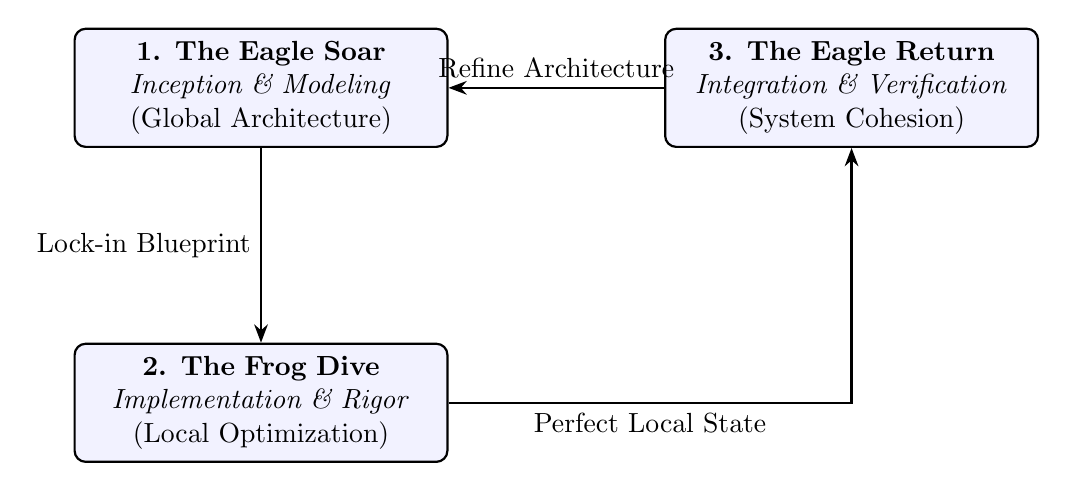
\begin{tikzpicture}[
		node distance=3cm,
		box/.style={rectangle, draw=black, thick, fill=blue!5, text width=4.5cm, align=center, rounded corners, minimum height=1.5cm},
		arrow/.style={thick, ->, >={Stealth}}
		]
		
		\node (eagle1) at (0, 0) [box] {\textbf{1. The Eagle Soar}\\ \textit{Inception \& Modeling}\\(Global Architecture)};
		\node (frog) at (0, -4) [box] {\textbf{2. The Frog Dive}\\ \textit{Implementation \& Rigor}\\(Local Optimization)};
		\node (eagle2) at (7.5, 0) [box] {\textbf{3. The Eagle Return}\\ \textit{Integration \& Verification}\\(System Cohesion)};
		
		\draw [arrow] (eagle1) -- (frog) node[midway, left] {Lock-in Blueprint};
		\draw [arrow] (frog) -| (eagle2) node[pos=0.25, below] {Perfect Local State};
		\draw [arrow] (eagle2) -- (eagle1) node[midway, above] {Refine Architecture};
	\end{tikzpicture}
	\caption{The Metamorphosis Cycle: Alternating between Eagle and Frog cognitive modes.}
\end{figure}

\begin{figure}[H]
	\centering
	\begin{tikzpicture}[
		node distance=3cm,
		box/.style={rectangle, draw=black, thick, fill=blue!5, text width=4.5cm, align=center, rounded corners, minimum height=1.5cm},
		arrow/.style={thick, ->, >={Stealth}}
		]
		
		\node (eagle1) at (0, 0) [box] {\textbf{1. Đại Bàng Bay Lượn}\\ \textit{Khởi đầu \& Lên mô hình}\\(Kiến trúc Toàn cục)};
		\node (frog) at (0, -4) [box] {\textbf{2. Cú Ngụp Lặn của Ếch}\\ \textit{Triển khai \& Khắt khe}\\(Tối ưu hóa Cục bộ)};
		\node (eagle2) at (7.5, 0) [box] {\textbf{3. Đại Bàng Trở Về}\\ \textit{Tích hợp \& Xác minh}\\(Sự Gắn kết Hệ thống)};
		
		\draw [arrow] (eagle1) -- (frog) node[midway, left] {Chốt Bản thiết kế};
		\draw [arrow] (frog) -| (eagle2) node[pos=0.25, below] {Hoàn thiện Trạng thái Cục bộ};
		\draw [arrow] (eagle2) -- (eagle1) node[midway, above] {Tinh chỉnh Kiến trúc};
	\end{tikzpicture}
	\caption{Bản dịch: Chu kỳ Biến hình: Sự luân phiên giữa các chế độ nhận thức Đại Bàng \& Ếch.}
\end{figure}

\begin{enumerate}[label=\emph{\arabic*.}]
	\item \emph{The Eagle Soar (Inception \& Modeling):} When tackling a complex research paper or a multi-layered optimization problem, you must ascend. You define the invariants, map out the combinatorial search space, and decide on the overarching strategy.
	
	\item \emph{Bản dịch - Đại Bàng Bay Lượn (Khởi đầu \& Lên mô hình):} Khi đương đầu với 1 bài báo nghiên cứu phức tạp hay 1 bài toán tối ưu hóa đa tầng, bạn phải bay lên. Bạn định nghĩa các bất biến, vẽ bản đồ không gian tìm kiếm tổ hợp, \& quyết định chiến lược bao quát.
	
	\begin{example}[AI Execution]
		Feed full documentation or core specs into a wide-context model (e.g., Gemini Flash / Extended) to scaffold the architecture.
	\end{example}
	\begin{vidu}[Thực thi với AI]
		Đưa toàn bộ tài liệu hoặc các đặc tả cốt lõi vào 1 mô hình có ngữ cảnh rộng (ví dụ: Gemini Flash / Extended) để tạo giàn giáo cho kiến trúc.
	\end{vidu}
	
	\item \emph{The Frog Dive (Implementation \& Rigor):} Once the blueprint is locked, you drop straight into the pond. You shut out the big picture and focus entirely on micro-optimization: core loops, edge cases, and strict mathematical rigor.
	
	\item \emph{Bản dịch - Cú Ngụp Lặn của Ếch (Triển khai \& Khắt khe):} Một khi bản thiết kế đã được chốt, bạn thả mình thẳng xuống ao. Bạn đóng sập cánh cửa với bức tranh toàn cảnh \& hoàn toàn tập trung vào việc tối ưu hóa vi mô: các vòng lặp cốt lõi, các trường hợp ngoại biên (edge cases), \& tính khắt khe nghiêm ngặt của toán học.
	
	\begin{example}[AI Execution]
		Shift to a high-precision reasoning model (e.g., Gemini Pro Deep Think) to verify tight mathematical bounds (such as evaluating precise $\lfloor r_{\text{opt}} \rfloor$ and $\lceil r_{\text{opt}} \rceil$ limits rather than loose search windows) and resolve subtle type conflicts.
	\end{example}
	\begin{vidu}[Thực thi với AI]
		Chuyển sang 1 mô hình lập luận có độ chính xác cao (ví dụ: Gemini Pro Deep Think) để xác minh các ranh giới toán học chặt chẽ (chẳng hạn như đánh giá các giới hạn $\lfloor r_{\text{opt}} \rfloor$ \& $\lceil r_{\text{opt}} \rceil$ chính xác thay vì các cửa sổ tìm kiếm lỏng lẻo) \& giải quyết các xung đột kiểu dữ liệu tinh vi.
	\end{vidu}
	
	\item \emph{The Eagle Return (Integration \& Verification):} After the local component is perfected, zoom back out to verify how your local optimization integrates with the global system state.
	
	\item \emph{Bản dịch - Đại Bàng Trở Về (Tích hợp \& Xác minh):} Sau khi thành phần cục bộ đã được hoàn thiện, hãy thu phóng góc nhìn ra xa trở lại để xác minh xem sự tối ưu hóa cục bộ của bạn tích hợp ra sao với trạng thái hệ thống toàn cục.
\end{enumerate}

\subsubsection{Cost of Shifting Perspectives}

\begin{remark}[Meta-Thinking Mode]
	The capability to shift between perspectives and mindsets is itself a distinct high-level perspective and mindset.
\end{remark}
\begin{nhanxet}[Chế độ Siêu Nhận Thức]
	Bản thân năng lực chuyển đổi giữa các góc nhìn \& tâm thế đã là 1 góc nhìn \& tâm thế cấp cao tách biệt.
\end{nhanxet}

Shapeshifting is cognitively expensive. Rapidly jumping between 30,000 feet and the granular details causes severe cognitive fatigue. We can mathematically formalize this cognitive friction. Let $S_t \in \{E, F\}$ denote the cognitive state (Eagle or Frog) at task step $t$. The total cognitive cost $C(\mathbf{S})$ over a sequence of $N$ tasks is given by the cost function:

Sự biến hình cực kỳ tốn kém về mặt nhận thức. Việc liên tục nhảy vọt giữa độ cao 30.000 feet \& những chi tiết dạng hạt gây ra sự mệt mỏi nhận thức nghiêm trọng. Chúng ta có thể hình thức hóa sự ma sát nhận thức này bằng toán học. Gọi $S_t \in \{E, F\}$ biểu thị trạng thái nhận thức (Đại Bàng hay Ếch) tại bước tác vụ $t$. Tổng chi phí nhận thức $C(\mathbf{S})$ qua 1 chuỗi $N$ tác vụ được cho bởi hàm chi phí:
\begin{equation}
	C(\mathbf{S}) = \sum_{t=1}^{N} c(S_t, \tau_t) + \lambda \sum_{t=1}^{N-1} \mathbf{1}_{\{S_t \neq S_{t+1}\}}
\end{equation}
where $c(S_t, \tau_t)$ is the baseline cognitive load of executing task $\tau_t$ in state $S_t$, $\mathbf{1}$ is the indicator function, and $\lambda \gg 0$ is the high switching penalty. The optimal workflow does not merely minimize instantaneous load; it must minimize state transitions. The solution lies in \textit{deliberate phase-locking}---forcing yourself to remain in the eagle state long enough to solidify system architecture before writing code (minimizing $\mathbf{1}_{\{S_t \neq S_{t+1}\}}$), and locking into the frog state long enough to reach deep flow without peripheral distractions.

trong đó $c(S_t, \tau_t)$ là tải nhận thức cơ sở khi thực thi tác vụ $\tau_t$ ở trạng thái $S_t$, $\mathbf{1}$ là hàm chỉ thị, \& $\lambda \gg 0$ là hình phạt chuyển đổi cao. Luồng công việc tối ưu không chỉ đơn thuần là giảm thiểu tải tức thời; nó phải giảm thiểu các lần chuyển đổi trạng thái. Giải pháp nằm ở \textit{sự khóa pha có chủ đích} (deliberate phase-locking)---ép buộc bản thân ở lại trạng thái đại bàng đủ lâu để củng cố vững chắc kiến trúc hệ thống trước khi bắt tay vào viết mã (giảm thiểu $\mathbf{1}_{\{S_t \neq S_{t+1}\}}$), \& khóa cứng vào trạng thái ếch đủ lâu để đạt tới trạng thái dòng chảy sâu (deep flow) mà không bị phân tâm bởi các yếu tố ngoại vi.

\begin{question}
	When designing a complex system or tackling an intricate algorithmic challenge, do you find yourself naturally anchored to one mode, forcing you to consciously fight your instincts to shift to the other?
\end{question}
\begin{cauhoi}
	Khi thiết kế 1 hệ thống phức tạp hoặc đương đầu với 1 thử thách thuật toán hóc búa, bạn có thấy mình tự nhiên thả neo vào 1 chế độ, buộc bản thân phải đấu tranh một cách có ý thức với bản năng để chuyển sang chế độ còn lại chăng?
\end{cauhoi}

%------------------------------------------------------------------------------%
\section*{Interlude: From Algorithms to Adversaries\\ Khúc Dạo Giữa: Từ Thuật toán đến Kẻ thù}
\addcontentsline{toc}{section}{Interlude: From Algorithms to Adversaries}
%------------------------------------------------------------------------------%

The Frog--Eagle dilemma fundamentally addresses optimization in cooperative, deterministic environments (e.g., codebases, mathematical proofs). However, real-world decision matrices rarely remain cooperative. When the environment shifts from a neutral landscape to an adversarial arena populated by malicious actors, pure intellectual optimization fails. The following sections transition from cognitive problem-solving to game-theoretic survival, mapping out decision frameworks for navigating high-conflict human dynamics where the standard assumption of mutual good faith ($U_{\text{empathy}} > 0$) collapses.

Thế tiến thoái lưỡng nan Ếch--Đại Bàng về cơ bản giải quyết bài toán tối ưu hóa trong các môi trường hợp tác, mang tính quyết định (ví dụ: kho mã nguồn, chứng minh toán học). Tuy nhiên, các ma trận quyết định trong thế giới thực hiếm khi nào giữ nguyên được tính hợp tác. Khi môi trường dịch chuyển từ 1 cảnh quan trung lập sang 1 đấu trường thù địch đầy rẫy những tác nhân ác ý, sự tối ưu hóa trí tuệ thuần túy sẽ thất bại. Các phần tiếp theo sẽ chuyển tiếp từ việc giải quyết vấn đề nhận thức sang sự sinh tồn theo lý thuyết trò chơi, vạch ra các bộ khung quyết định nhằm lèo lái qua những động lực tương tác con người đầy xung đột, nơi mà giả định tiêu chuẩn về sự thiện ý lẫn nhau ($U_{\text{empathy}} > 0$) hoàn toàn sụp đổ.

%------------------------------------------------------------------------------%
\section{Some Psychological Decision Problems}
%------------------------------------------------------------------------------%

\subsection{The dark triad \& sociopath}

\begin{question}[Navigating High-Conflict \& Narcissistic Dynamics]
	When encountering highly manipulative or narcissistic individuals, what immediate tactical decision problems must be resolved to protect personal, professional, and psychological integrity?
\end{question}
\begin{cauhoi}[Lèo lái qua các Động lực Xung đột Cao \& Ái kỷ]
	Khi đụng độ những cá nhân ái kỷ hoặc có tính thao túng cao, những bài toán quyết định chiến thuật tức thời nào phải được giải quyết để bảo vệ sự toàn vẹn về mặt cá nhân, sự nghiệp, \& tâm lý?
\end{cauhoi}

Standard assumptions of mutual good faith and reciprocal negotiation break down in these settings. Because their behavior is driven by a need for control, validation, or dominance, high-stakes tactical decisions must be made rapidly.

Các giả định tiêu chuẩn về thiện ý lẫn nhau \& sự đàm phán có đi có lại hoàn toàn tan vỡ trong những bối cảnh này. Bởi lẽ hành vi của họ được thúc đẩy bởi nhu cầu kiểm soát, sự khao khát được công nhận, hay sự thống trị, những quyết định chiến thuật mang tính rủi ro cao phải được đưa ra 1 cách chớp nhoáng.

\begin{problem}[Engagement Boundary: Zero-Contact vs. Transactional Shielding]
	\emph{Core Dilemma:} Deciding immediately how much access this individual is granted.
	\begin{enumerate}[label=(\roman*)]
		\item \emph{Decision Strategy:} Rapidly assess whether complete elimination of contact (zero-contact) is viable, or if shared institutional/departmental environments necessitate a \textit{low-contact, strictly transactional} protocol (the Gray Rock method).
		\item \emph{Trade-off:} Delaying this decision allows the individual to establish psychological leverage or operational entanglement, making subsequent separation exponentially more costly.
	\end{enumerate}
\end{problem}
\begin{baitoan}[Ranh giới Tương tác: Không Tiếp xúc vs. Lá chắn Giao dịch]
	\emph{Thế Tiến thoái Lưỡng nan Cốt lõi:} Quyết định ngay lập tức mức độ quyền truy cập mà cá nhân này được ban cấp.
	\begin{enumerate}[label=(\roman*)]
		\item \emph{Chiến lược Quyết định:} Đánh giá chớp nhoáng xem liệu việc loại bỏ hoàn toàn liên lạc (không tiếp xúc - zero-contact) có khả thi hay không, hoặc liệu các môi trường chung (tổ chức/phòng ban) có bắt buộc phải áp dụng 1 giao thức \textit{tiếp xúc thấp, thuần túy giao dịch} hay không (phương pháp Đá Xám - Gray Rock).
		\item \emph{Sự Đánh đổi:} Việc trì hoãn quyết định này tạo điều kiện cho cá nhân kia thiết lập đòn bẩy tâm lý hoặc sự vướng mắc vận hành, khiến cho việc chia tách sau đó trở nên đắt đỏ theo cấp số nhân.
	\end{enumerate}
\end{baitoan}

\begin{problem}[Information Asymmetry: Exposure vs. Vulnerability Shielding]
	\emph{Core Dilemma:} Determining the permissible depth of personal and intellectual disclosure.
	\begin{enumerate}[label=(\roman*)]
		\item \emph{Decision Strategy:} Immediately halt all non-essential personal disclosures. Manipulative actors actively scan for vulnerabilities, career ambitions, or insecurities to exploit in future devaluation phases.
		\item \emph{Trade-off:} While natural professional relationships thrive on candor, interaction in high-conflict settings requires restricting exchanges to objective, uninteresting, and purely factual statements.
	\end{enumerate}
\end{problem}
\begin{baitoan}[Bất đối xứng Thông tin: Phơi bày vs. Che chắn Khuyết điểm]
	\emph{Thế Tiến thoái Lưỡng nan Cốt lõi:} Xác định độ sâu cho phép của việc bộc lộ cá nhân \& tri thức.
	\begin{enumerate}[label=(\roman*)]
		\item \emph{Chiến lược Quyết định:} Ngay lập tức đình chỉ mọi sự bộc lộ cá nhân không thiết yếu. Các tác nhân thao túng luôn chủ động rà quét các điểm yếu, tham vọng sự nghiệp, hoặc những sự bất an để trục lợi trong các giai đoạn hạ giá (devaluation) trong tương lai.
		\item \emph{Sự Đánh đổi:} Dẫu cho những mối quan hệ công việc thuận tự nhiên thăng hoa dựa trên sự vô tư, chân thật, thì việc tương tác trong các bối cảnh xung đột cao lại đòi hỏi phải giới hạn các cuộc trao đổi vào những phát ngôn khách quan, nhạt nhẽo, \& thuần túy là dữ kiện thực tế.
	\end{enumerate}
\end{baitoan}

\begin{problem}[Conflict Trigger: Fact Correction vs. Escalation Containment]
	\emph{Core Dilemma:} Deciding whether to publicly refute distortions or allow false narratives to pass uncorrected.
	\begin{enumerate}[label=(\roman*)]
		\item \emph{Decision Strategy:} Choose between immediate truth-seeking and long-term resource preservation. Direct public correction often triggers disproportionate defensive reactions or protracted mudslinging.
		\item \emph{Trade-off:} Correcting every misstatement drains cognitive bandwidth; however, total passivity risks letting false narratives become accepted precedent. Selective, documented correction is required.
	\end{enumerate}
\end{problem}
\begin{baitoan}[Kích hoạt Xung đột: Chỉnh lý Sự thật vs. Kìm hãm Leo thang]
	\emph{Thế Tiến thoái Lưỡng nan Cốt lõi:} Quyết định xem nên công khai bác bỏ những sự xuyên tạc hay cứ mặc cho những tường thuật dối trá trôi qua mà không thèm chỉnh lý.
	\begin{enumerate}[label=(\roman*)]
		\item \emph{Chiến lược Quyết định:} Lựa chọn giữa việc truy tìm sự thật tức thời \& việc bảo tồn tài nguyên dài hạn. Sự chỉnh lý công khai, trực diện thường kích hoạt những phản ứng phòng vệ thái quá hoặc những màn ném bùn kéo dài dai dẳng.
		\item \emph{Sự Đánh đổi:} Việc chỉnh lý mọi phát ngôn sai lệch sẽ vắt kiệt băng thông nhận thức; dẫu vậy, sự bị động hoàn toàn lại mang rủi ro để cho những câu chuyện dối trá trở thành tiền lệ được chấp nhận. Một sự chỉnh lý có chọn lọc, được lưu trữ văn bản là điều tối thiết.
	\end{enumerate}
\end{baitoan}

\begin{problem}[Evidence Preservation: Verbal Trust vs. Paper Trail Protocol]
	\emph{Core Dilemma:} Choosing between informal peer agreements and strict written documentation.
	\begin{enumerate}[label=(\roman*)]
		\item \emph{Decision Strategy:} Instantly transition to an \textit{assume-bad-faith protocol}, ensuring every project scope, task allocation, and commitment is recorded in unambiguous written form (e.g., follow-up emails, written specifications).
		\item \emph{Trade-off:} Operating with strict paper trails may feel overly bureaucratic to standard peers, but it serves as the sole defense against gaslighting, credit theft, and retrospective narrative revision.
	\end{enumerate}
\end{problem}
\begin{baitoan}[Bảo tồn Bằng chứng: Niềm tin Lời nói vs. Giao thức Dấu vết Giấy tờ]
	\emph{Thế Tiến thoái Lưỡng nan Cốt lõi:} Lựa chọn giữa những thỏa thuận đồng nghiệp phi chính thức \& sự lưu trữ tài liệu văn bản nghiêm ngặt.
	\begin{enumerate}[label=(\roman*)]
		\item \emph{Chiến lược Quyết định:} Chuyển sang \textit{giao thức giả định ác ý} ngay lập tức, đảm bảo rằng mọi phạm vi dự án, phân bổ tác vụ, \& cam kết đều được ghi chép lại dưới dạng văn bản không thể nhập nhằng (ví dụ: email theo dõi, đặc tả văn bản).
		\item \emph{Sự Đánh đổi:} Việc vận hành với những dấu vết giấy tờ (paper trails) nghiêm ngặt có thể tạo cảm giác quá sức quan liêu đối với các đồng nghiệp thông thường, nhưng nó đóng vai trò là hàng phòng ngự duy nhất chống lại chiêu trò thao túng tâm lý (gaslighting), đánh cắp công trạng, \& việc hồi tố sửa đổi câu chuyện.
	\end{enumerate}
\end{baitoan}

\begin{problem}[Triangulation \& Coalition Defense: Passive Neutrality vs. Strategic Visibility]
	\emph{Core Dilemma:} Managing third-party manipulation and subterranean smear efforts.
	\begin{enumerate}[label=(\roman*)]
		\item \emph{Decision Strategy:} Decide whether to proactively inform key stakeholders or maintain a dignified, neutral posture while demonstrating consistency over time.
		\item \emph{Trade-off:} Proactive self-defense risks appearing overly defensive or dramatic, whereas complete silence allows manipulative narratives to establish an unchallenged foothold.
	\end{enumerate}
\end{problem}
\begin{baitoan}[Tam giác hóa \& Phòng thủ Liên minh: Trung lập Bị động vs. Sự Hiện diện Chiến lược]
	\emph{Thế Tiến thoái Lưỡng nan Cốt lõi:} Xử lý sự thao túng bên thứ ba \& những nỗ lực bôi nhọ ngầm.
	\begin{enumerate}[label=(\roman*)]
		\item \emph{Chiến lược Quyết định:} Quyết định xem nên chủ động thông báo cho các bên liên quan then chốt hay duy trì 1 tư thế trung lập, đĩnh đạc trong khi chứng minh tính nhất quán theo thời gian.
		\item \emph{Sự Đánh đổi:} Sự tự vệ chủ động mang nguy cơ tạo vẻ bề ngoài quá phòng thủ hay bi kịch hóa, trong khi sự im lặng tuyệt đối lại cho phép những câu chuyện thao túng thiết lập 1 chỗ đứng không thể bị thách thức.
	\end{enumerate}
\end{baitoan}

%------------------------------------------------------------------------------%
\subsection{Antisocial dynamics}
%------------------------------------------------------------------------------%

\begin{question}[Navigating Sociopathic \& Psychopathic Dynamics]
	When encountering sociopathic or psychopathic individuals, what immediate tactical decision problems must be resolved to protect personal, operational, and institutional integrity?
\end{question}
\begin{cauhoi}[Lèo lái qua các Động lực Rối loạn Nhân cách Chống đối Xã hội \& Ái kỷ]
	Khi đụng độ những cá nhân rối loạn nhân cách chống đối xã hội (sociopathic) hay rối loạn nhân cách chống đối xã hội bẩm sinh (psychopathic), những bài toán quyết định chiến thuật tức thời nào phải được giải quyết để bảo vệ sự toàn vẹn về mặt cá nhân, vận hành, \& thể chế?
\end{cauhoi}

Unlike narcissists, who operate to preserve ego and secure admiration, antisocial actors exhibit a total deficit of affective empathy. Sociopaths are characterized by emotional volatility and impulsive rule-breaking, whereas psychopaths execute cold, calculated, and instrumental predation. Standard social contracts and reputation-based deterrence fail completely in these regimes.

Khác với những kẻ ái kỷ, những người vận hành nhằm mục đích bảo tồn cái tôi \& củng cố sự ngưỡng mộ, các tác nhân chống đối xã hội (antisocial) phô bày 1 sự khuyết thiếu hoàn toàn về sự thấu cảm xúc cảm (affective empathy). Sociopaths được đặc trưng bởi sự biến động cảm xúc \& sự phá vỡ luật lệ bốc đồng, trong khi psychopaths lại thi triển những màn săn mồi lạnh lùng, đầy toan tính, \& mang tính công cụ. Những bản hợp đồng xã hội tiêu chuẩn \& sự răn đe dựa trên danh tiếng hoàn toàn sụp đổ trong các chế độ này.

\begin{problem}[Threat Categorization: Volatile Chaos vs. Instrumental Predation]
	\emph{Core Dilemma:} Rapidly identifying whether the adversary is driven by erratic impulse (sociopathy) or calculated utility maximization (psychopathy).
	\begin{enumerate}[label=(\roman*)]
		\item \emph{Decision Strategy:} Evaluate behavioral signatures. Determine if hostility is explosive and reactive or smooth, charming, and targeted toward long-term asset capture.
		\item \emph{Trade-off:} Misdiagnosing a psychopath as merely volatile leaves one blind to multi-stage predatory traps; misdiagnosing a sociopath as a master strategist wastes energy preparing for complex plots when simple physical or operational containment is required.
	\end{enumerate}
\end{problem}
\begin{baitoan}[Phân loại Mối đe dọa: Sự Hỗn loạn Biến động vs. Cuộc Săn mồi Công cụ]
	\emph{Thế Tiến thoái Lưỡng nan Cốt lõi:} Xác định chớp nhoáng xem liệu kẻ thù bị thôi thúc bởi những xung lực bốc đồng, thất thường (sociopathy) hay sự tối đa hóa hữu dụng mang tính toan tính (psychopathy).
	\begin{enumerate}[label=(\roman*)]
		\item \emph{Chiến lược Quyết định:} Đánh giá các dấu hiệu hành vi. Định đoạt xem liệu sự thù địch mang tính bùng nổ \& phản xạ, hay trơn tru, đầy mê hoặc, \& nhắm mục tiêu vào sự tước đoạt tài sản dài hạn.
		\item \emph{Sự Đánh đổi:} Chẩn đoán sai 1 psychopath chỉ đơn thuần là 1 kẻ hay biến động sẽ khiến ta mù lòa trước những chiếc bẫy săn mồi đa giai đoạn; chẩn đoán sai 1 sociopath thành 1 bậc thầy chiến lược sẽ làm hao phí sinh lực để chuẩn bị cho những âm mưu phức tạp trong khi thứ duy nhất được yêu cầu chỉ là 1 sự phong tỏa vật lý hay vận hành đơn giản.
	\end{enumerate}
\end{baitoan}

\begin{problem}[Egress Strategy: Managed De-escalation vs. Silent Extraction]
	\emph{Core Dilemma:} Choosing the optimal protocol for severing operational or personal ties without triggering explosive retaliation.
	
	This scenario can be modeled as an extensive-form game, illustrating the strategic divergence between facing a reactive Sociopath versus a calculating Psychopath:
	
	\begin{figure}[H]
		\centering
		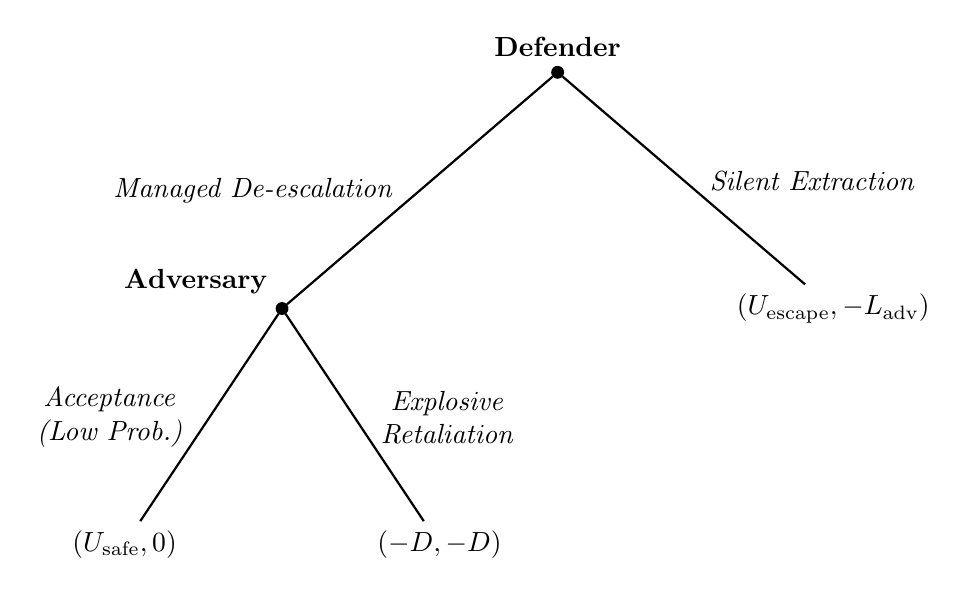
\begin{tikzpicture}[
			level 1/.style={sibling distance=7cm, level distance=3cm},
			level 2/.style={sibling distance=4cm, level distance=3cm},
			solid node/.style={circle,draw,inner sep=1.5pt,fill=black},
			edge from parent/.style={thick, draw}
			]
			
			\node[solid node, label=above:{\textbf{Defender}}] {}
			child { node[solid node, label=above left:{\textbf{Adversary}}] {}
				child { node {$(U_{\text{safe}}, 0)$} 
					edge from parent node[left, align=center, xshift=-0.2cm] {\emph{Acceptance}\\\emph{(Low Prob.)}} 
				}
				child { node {$(-D, -D)$} 
					edge from parent node[right, align=center, xshift=0.2cm] {\emph{Explosive}\\\emph{Retaliation}} 
				}
				edge from parent node[left, xshift=-0.2cm] {\emph{Managed De-escalation}}
			}
			child { node {$(U_{\text{escape}}, -L_{\text{adv}})$}
				edge from parent node[right, xshift=0.2cm] {\emph{Silent Extraction}}
			};
		\end{tikzpicture}
		\caption{Extensive-form game tree for Egress Strategy. \emph{Managed De-escalation} hands the move to the adversary, risking explosive retaliation (cost $-D$). \emph{Silent Extraction} bypasses the adversary's decision node entirely, guaranteeing escape (payoff $U_{\text{escape}}$) while inflicting a loss on the adversary ($-L_{\text{adv}}$) without retaliation.}
	\end{figure}
	
	\begin{enumerate}[label=(\roman*)]
		\item \emph{Decision Strategy:} Apply gradual, low-energy decoupling to volatile sociopaths to avoid triggering explosive rage. For calculating psychopaths, execute \textit{silent, zero-warning extraction}---severing access completely before the strategic intent is signaled.
		\item \emph{Trade-off:} Telegraphing exit plans gives a psychopath time to lock down resources or pre-emptively sabotage the target; abrupt exits with a sociopath can trigger immediate, volatile confrontations.
	\end{enumerate}
\end{problem}
\begin{baitoan}[Chiến lược Thoát hiểm: Khử leo thang Có quản lý vs. Giải cứu Lặng lẽ]
	\emph{Thế Tiến thoái Lưỡng nan Cốt lõi:} Lựa chọn giao thức tối ưu để cắt đứt các mối liên hệ vận hành hay cá nhân mà không kích hoạt sự trả đũa bùng nổ.
	
	Kịch bản này có thể được mô hình hóa như 1 trò chơi dạng mở rộng (extensive-form game), minh họa sự phân kỳ chiến lược giữa việc đối mặt với 1 Sociopath phản xạ so với 1 Psychopath đầy toan tính:
	
	\begin{figure}[H]
		\centering
		\begin{tikzpicture}[
			level 1/.style={sibling distance=7cm, level distance=3cm},
			level 2/.style={sibling distance=4cm, level distance=3cm},
			solid node/.style={circle,draw,inner sep=1.5pt,fill=black},
			edge from parent/.style={thick, draw}
			]
			
			\node[solid node, label=above:{\textbf{Người phòng thủ}}] {}
			child { node[solid node, label=above left:{\textbf{Kẻ thù}}] {}
				child { node {$(U_{\text{safe}}, 0)$} 
					edge from parent node[left, align=center, xshift=-0.2cm] {\emph{Chấp nhận}\\\emph{(Xác suất thấp)}} 
				}
				child { node {$(-D, -D)$} 
					edge from parent node[right, align=center, xshift=0.2cm] {\emph{Trả đũa}\\\emph{Bùng nổ}} 
				}
				edge from parent node[left, xshift=-0.2cm] {\emph{Khử leo thang Có quản lý}}
			}
			child { node {$(U_{\text{escape}}, -L_{\text{adv}})$}
				edge from parent node[right, xshift=0.2cm] {\emph{Giải cứu Lặng lẽ}}
			};
		\end{tikzpicture}
		\caption{Bản dịch: Cây trò chơi dạng mở rộng cho Chiến lược Thoát hiểm. \emph{Khử leo thang Có quản lý} trao nước đi cho kẻ thù, mang rủi ro trả đũa bùng nổ (chi phí $-D$). \emph{Giải cứu Lặng lẽ} đi vòng qua điểm quyết định của kẻ thù hoàn toàn, đảm bảo sự trốn thoát (phần thưởng $U_{\text{escape}}$) đồng thời giáng 1 tổn thất lên kẻ thù ($-L_{\text{adv}}$) mà không có sự trả đũa.}
	\end{figure}
	
	\begin{enumerate}[label=(\roman*)]
		\item \emph{Chiến lược Quyết định:} Áp dụng sự tách rời dần dần, tiêu hao năng lượng thấp đối với những sociopaths hay biến động để tránh kích hoạt cơn thịnh nộ bùng nổ. Đối với những psychopaths đầy toan tính, thi triển \textit{sự giải cứu lặng lẽ, không cảnh báo}---cắt đứt quyền truy cập hoàn toàn trước khi ý định chiến lược bị phát đi.
		\item \emph{Sự Đánh đổi:} Việc đánh điện tín các kế hoạch rời đi sẽ cho 1 psychopath thời gian để khóa chặt các tài nguyên hay chủ động phá hoại mục tiêu từ trước; những sự rời đi đột ngột với 1 sociopath có thể kích hoạt những cuộc đối đầu biến động, ngay lập tức.
	\end{enumerate}
\end{baitoan}

\begin{problem}[Incentive Design: Moral Appeals vs. Algorithmic Constraints]
	\emph{Core Dilemma:} Establishing operational control when emotional leverage, shared history, and social norms carry zero utility ($U_{\text{empathy}} = 0$).
	
	To formalize this dynamic, consider a normal-form game between a Defender and an Antisocial Actor. Standard mutual cooperation \cite{axelrod1984evolution} relies on the actor suffering an internal moral penalty. When this penalty is absent, we obtain the following payoff matrix:
	
	\begin{table}[H]
		\centering
		\renewcommand{\arraystretch}{1.5}
		\begin{tabular}{r|c|c|}
			\multicolumn{1}{c}{} & \multicolumn{1}{c}{\emph{Actor: Comply}} & \multicolumn{1}{c}{\emph{Actor: Defect}} \\ \cline{2-3}
			\emph{Defender: Moral Appeal} & $(0, 0)$ & $(-L, +G)$ \\ \cline{2-3}
			\emph{Defender: Algorithmic Constraint} & $(-c, 0)$ & $(-c, -P)$ \\ \cline{2-3}
		\end{tabular}
		\caption{Payoff matrix where $L \gg c$ is the Defender's loss from exploitation, $G > 0$ is the Actor's gain from defection, $c > 0$ is the cost of implementing hard constraints, and $P > G$ is the enforced deterministic penalty for defection.}
	\end{table}
	
	\begin{enumerate}[label=(\roman*)]
		\item \emph{Decision Strategy:} Abandon moral appeals entirely. Construct rigid game-theoretic environments where compliance is enforced purely through deterministic costs, hard system access locks, and immutable audits (playing \emph{Algorithmic Constraint}).
		\item \emph{Trade-off:} Relying on goodwill guarantees defection because \emph{Defect} strictly dominates \emph{Comply} for the actor when facing a \emph{Moral Appeal} (since $G > 0$). Hardening system constraints requires continuous overhead and enforcement (cost $-c$), as defection will occur the precise moment the penalty condition fails. This alters the actor's payoff from $+G$ to $-P$, enforcing compliance as the rational response.
	\end{enumerate}
\end{problem}
\begin{baitoan}[Thiết kế Động cơ: Lời Kêu gọi Đạo đức vs. Ràng buộc Thuật toán]
	\emph{Thế Tiến thoái Lưỡng nan Cốt lõi:} Thiết lập quyền kiểm soát vận hành khi đòn bẩy cảm xúc, lịch sử chung, \& các chuẩn mực xã hội mang giá trị hữu dụng bằng không ($U_{\text{empathy}} = 0$).
	
	Để hình thức hóa động lực này, hãy xem xét 1 trò chơi dạng chuẩn (normal-form game) giữa 1 Người phòng thủ \& 1 Tác nhân Chống đối Xã hội. Sự hợp tác lẫn nhau tiêu chuẩn \cite{axelrod1984evolution} dựa dẫm vào việc tác nhân phải gánh chịu 1 hình phạt đạo đức nội tâm. Khi hình phạt này vắng mặt, ta thu được ma trận phần thưởng sau:
	
	\begin{table}[H]
		\centering
		\renewcommand{\arraystretch}{1.5}
		\begin{tabular}{r|c|c|}
			\multicolumn{1}{c}{} & \multicolumn{1}{c}{\emph{Tác nhân: Tuân thủ}} & \multicolumn{1}{c}{\emph{Tác nhân: Phản bội}} \\ \cline{2-3}
			\emph{Phòng thủ: Kêu gọi Đạo đức} & $(0, 0)$ & $(-L, +G)$ \\ \cline{2-3}
			\emph{Phòng thủ: Ràng buộc Thuật toán} & $(-c, 0)$ & $(-c, -P)$ \\ \cline{2-3}
		\end{tabular}
		\caption{Bản dịch: Ma trận phần thưởng trong đó $L \gg c$ là tổn thất của Người phòng thủ từ việc bị bóc lột, $G > 0$ là món lợi của Tác nhân từ sự phản bội, $c > 0$ là chi phí của việc thực thi các ràng buộc cứng, \& $P > G$ là hình phạt mang tính quyết định, bị ép buộc dành cho sự phản bội.}
	\end{table}
	
	\begin{enumerate}[label=(\roman*)]
		\item \emph{Chiến lược Quyết định:} Từ bỏ hoàn toàn các lời kêu gọi đạo đức. Kiến tạo các môi trường lý thuyết trò chơi cứng nhắc nơi sự tuân thủ bị ép buộc thuần túy thông qua các chi phí mang tính quyết định, các khóa truy cập hệ thống cứng, \& những sự kiểm toán bất biến (chọn nước đi \emph{Ràng buộc Thuật toán}).
		\item \emph{Sự Đánh đổi:} Dựa dẫm vào thiện ý đảm bảo 1 sự phản bội bởi lẽ \emph{Phản bội} áp đảo hoàn toàn (strictly dominates) \emph{Tuân thủ} đối với tác nhân khi đối mặt với \emph{Kêu gọi Đạo đức} (vì $G > 0$). Việc làm cứng các ràng buộc hệ thống đòi hỏi chi phí chìm \& sự thực thi liên tục (chi phí $-c$), bởi lẽ sự phản bội sẽ xảy ra vào đúng khoảnh khắc điều kiện hình phạt thất bại. Điều này đảo ngược phần thưởng của tác nhân từ $+G$ thành $-P$, ép buộc sự tuân thủ như 1 phản ứng hợp lý.
	\end{enumerate}
\end{baitoan}

\begin{problem}[Charisma Filtering: Superficial Alignment vs. Zero-Trust Verification]
	\emph{Core Dilemma:} Maintaining analytical objectivity against smooth, highly charming actors who mirror expectations perfectly.
	\begin{enumerate}[label=(\roman*)]
		\item \emph{Decision Strategy:} Enforce a strict \textit{Zero-Trust Verification Protocol}. Ignore interpersonal rapport, authority claims, or verbal commitments; evaluate alignment exclusively through verifiable logs, hard data, and independent third-party checks.
		\item \emph{Trade-off:} Auditing a charismatic peer risks provoking skepticism or social friction from naive third parties who remain captivated by the surface facade.
	\end{enumerate}
\end{problem}
\begin{baitoan}[Lọc Sự Lôi cuốn: Gióng hàng Hời hợt vs. Xác minh Không Niềm tin]
	\emph{Thế Tiến thoái Lưỡng nan Cốt lõi:} Duy trì tính khách quan phân tích trước những tác nhân trơn tru, cực kỳ duyên dáng, những kẻ phản chiếu các kỳ vọng 1 cách hoàn mỹ.
	\begin{enumerate}[label=(\roman*)]
		\item \emph{Chiến lược Quyết định:} Thực thi 1 \textit{Giao thức Xác minh Không Niềm tin (Zero-Trust)} nghiêm ngặt. Phớt lờ sự hòa hợp cá nhân, những tuyên bố uy quyền, hay những cam kết bằng lời nói; đánh giá sự gióng hàng độc quyền thông qua các nhật ký (logs) có thể kiểm chứng, dữ liệu cứng, \& sự kiểm tra độc lập từ bên thứ ba.
		\item \emph{Sự Đánh đổi:} Kiểm toán 1 đồng nghiệp lôi cuốn mang nguy cơ khiêu khích sự hoài nghi hay sự ma sát xã hội từ những bên thứ ba ngây thơ, những người vẫn đang bị mê hoặc bởi lớp mặt nạ bề ngoài.
	\end{enumerate}
\end{baitoan}

\begin{problem}[Systemic Inoculation: Whistleblowing vs. Private Survival]
	\emph{Core Dilemma:} Balancing the ethical duty to protect the broader organization against the severe risks of direct confrontation.
	\begin{enumerate}[label=(\roman*)]
		\item \emph{Decision Strategy:} Evaluate organizational capture. If institutional leadership is compromised or oblivious, secure complete personal decoupling before initiating external exposure.
		\item \emph{Trade-off:} Active whistleblowing invites scorched-earth retaliation (legal attacks, targeted sabotage); quiet extraction guarantees personal safety but leaves the surrounding environment vulnerable to predation.
	\end{enumerate}
\end{problem}
\begin{baitoan}[Tiêm chủng Hệ thống: Thổi còi vs. Sinh tồn Cá nhân]
	\emph{Thế Tiến thoái Lưỡng nan Cốt lõi:} Cân bằng giữa nghĩa vụ đạo đức bảo vệ tổ chức rộng lớn hơn \& những rủi ro khốc liệt của cuộc đối đầu trực diện.
	\begin{enumerate}[label=(\roman*)]
		\item \emph{Chiến lược Quyết định:} Đánh giá sự thâu tóm tổ chức (organizational capture). Nếu giới lãnh đạo thể chế đã bị thỏa hiệp hoặc làm ngơ, hãy bảo đảm 1 sự tách rời cá nhân hoàn toàn trước khi khởi xướng bất kỳ sự phơi bày ngoại vi nào.
		\item \emph{Sự Đánh đổi:} Sự thổi còi (whistleblowing) chủ động mời gọi 1 sự trả đũa theo chiến thuật tiêu thổ (các cuộc tấn công pháp lý, sự phá hoại có chủ đích); sự giải cứu lặng lẽ đảm bảo an toàn cá nhân nhưng lại bỏ mặc môi trường xung quanh cho những chiếc bẫy săn mồi.
	\end{enumerate}
\end{baitoan}

%------------------------------------------------------------------------------%
\section{Some Philosophical Decision Problems}
%------------------------------------------------------------------------------%

Philosophical decision-making often presents a stark contrast between existential agency and pragmatic duty. While academic and interpersonal problems map readily to discrete optimization, existential choices involve undefined utility functions and infinite horizons.

Việc ra quyết định triết học thường phơi bày 1 sự tương phản sắc nét giữa tính tác nhân sinh tồn (existential agency) \& nghĩa vụ thực chứng. Trong khi các bài toán học thuật \& tương tác cá nhân có thể dễ dàng ánh xạ vào sự tối ưu hóa rời rạc, thì những lựa chọn sinh tồn (existential choices) lại bao hàm những hàm hữu dụng không được định nghĩa \& những chân trời vô hạn.

\begin{problem}[The Existential Commitment Problem]
	\emph{Core Dilemma:} Choosing between a Kierkegaardian existential leap \cite{kierkegaard1843fear} (acting under fundamental uncertainty) and pragmatic systemic alignment.
	\begin{enumerate}[label=(\roman*)]
		\item \emph{Decision Strategy:} Establish explicit stopping criteria for decision analysis (a meta-decision) to prevent endless philosophical paralysis. Treat the existential leap not as a blind guess, but as an $\varepsilon$-greedy exploration step where $\varepsilon$ scales with life dissatisfaction.
		\item \emph{Trade-off:} Over-analyzing philosophical alignment stalls execution and wastes finite biological time, while hasty commitment without core alignment leads to long-term existential dissonance.
	\end{enumerate}
\end{problem}
\begin{baitoan}[Bài toán Cam kết Sinh tồn]
	\emph{Thế Tiến thoái Lưỡng nan Cốt lõi:} Lựa chọn giữa bước nhảy vọt sinh tồn mang phong cách Kierkegaard \cite{kierkegaard1843fear} (hành động dưới sự bất định nền tảng) \& sự gióng hàng hệ thống thực chứng.
	\begin{enumerate}[label=(\roman*)]
		\item \emph{Chiến lược Quyết định:} Thiết lập các tiêu chí dừng hiển ngôn cho việc phân tích quyết định (một siêu quyết định) nhằm ngăn chặn sự tê liệt triết học vô tận. Đừng coi bước nhảy vọt sinh tồn như 1 sự suy đoán mù quáng, mà hãy xem nó như 1 bước khám phá $\varepsilon$-tham lam ($\varepsilon$-greedy) nơi $\varepsilon$ tỷ lệ thuận với sự bất mãn cuộc sống.
		\item \emph{Sự Đánh đổi:} Phân tích quá mức sự gióng hàng triết học sẽ làm đình trệ sự thực thi \& lãng phí thời gian sinh học hữu hạn, trong khi sự cam kết vội vã mà không có sự gióng hàng cốt lõi sẽ dẫn đến sự bất hòa sinh tồn (existential dissonance) dài hạn.
	\end{enumerate}
\end{baitoan}

%------------------------------------------------------------------------------%
\section{Some Life Decision Problems}
%------------------------------------------------------------------------------%

Life decisions fundamentally reduce to multidimensional resource allocation problems under strict biological constraints (time, energy, cognitive bandwidth).

Những quyết định cuộc đời về cơ bản thu gọn lại thành các bài toán phân bổ tài nguyên đa chiều dưới những ràng buộc sinh học nghiêm ngặt (thời gian, năng lượng, băng thông nhận thức).

\begin{problem}[Resource Allocation: Solitude vs. Integration]
	\emph{Core Dilemma:} Balancing personal creative/scientific sovereignty with domestic and social obligations under constrained cognitive bandwidth.
	\begin{enumerate}[label=(\roman*)]
		\item \emph{Decision Strategy:} Treat cognitive bandwidth as a strictly bounded, non-renewable daily resource. If an individual cannot fully sustain the financial, emotional, and temporal requirements of a family or social unit without degrading core research/creative outputs below a viable threshold, prioritizing purposeful solitude becomes the optimal default.
		\item \emph{Trade-off:} Choosing solitude requires sacrificing traditional social support structures and long-term domestic stability, but in return, it preserves unconditional autonomy and maximum unbroken flow-states for intellectual focus.
	\end{enumerate}
\end{problem}
\begin{baitoan}[Phân bổ Tài nguyên: Sự Cô độc vs. Sự Hội nhập]
	\emph{Thế Tiến thoái Lưỡng nan Cốt lõi:} Cân bằng giữa chủ quyền sáng tạo/khoa học cá nhân \& các nghĩa vụ nội bộ và xã hội dưới sự hạn chế của băng thông nhận thức.
	\begin{enumerate}[label=(\roman*)]
		\item \emph{Chiến lược Quyết định:} Xem băng thông nhận thức như 1 nguồn tài nguyên hằng ngày bị giới hạn nghiêm ngặt, không thể tái tạo. Nếu 1 cá nhân không thể duy trì trọn vẹn các yêu cầu về tài chính, cảm xúc, \& thời gian của 1 gia đình hay 1 đơn vị xã hội mà không làm suy thoái các sản phẩm nghiên cứu/sáng tạo cốt lõi xuống dưới mức ngưỡng khả thi, thì việc ưu tiên 1 sự cô độc có chủ đích sẽ trở thành mặc định tối ưu.
		\item \emph{Sự Đánh đổi:} Lựa chọn sự cô độc đòi hỏi phải hy sinh các cấu trúc hỗ trợ xã hội truyền thống \& sự ổn định nội bộ dài hạn, nhưng đổi lại, nó bảo tồn sự tự chủ vô điều kiện \& các trạng thái dòng chảy không bị đứt đoạn tối đa dành cho sự tập trung trí tuệ.
	\end{enumerate}
\end{baitoan}

\begin{problem}[The Explore/Exploit Tradeoff in Career Trajectories]
	\emph{Core Dilemma:} Deciding whether to sample new, high-variance professional domains (exploration) or to maximize compounding returns within a known, specialized trajectory (exploitation). This maps formally to a Multi-Armed Bandit (MAB) problem, where one must allocate finite biological time ($T$) across various career ``arms'' with unknown payoff distributions.
	\begin{enumerate}[label=(\roman*)]
		\item \emph{Decision Strategy:} Implement an Upper Confidence Bound (UCB) algorithm or an $\varepsilon$-greedy heuristic over the career timeline. In the early phases ($t \ll T$), aggressively explore high-variance domains to maximize information gain. As time progresses ($t \to T$), deterministically shift to exploiting the arm yielding the highest expected reward, thereby minimizing cumulative regret.
		\item \emph{Trade-off:} Perpetual exploration avoids local optima but risks resulting in a fragmented trajectory with negligible compounding capital. Conversely, premature exploitation ensures steady, compounding returns but risks committing to a sub-optimal local maximum, incurring severe opportunity cost if a vastly superior, undiscovered path existed.
	\end{enumerate}
\end{problem}
\begin{baitoan}[Sự Đánh đổi Khám phá/Khai thác trong Quỹ đạo Sự nghiệp]
	\emph{Thế Tiến thoái Lưỡng nan Cốt lõi:} Quyết định xem nên lấy mẫu những miền chuyên môn mới, có phương sai cao (khám phá) hay tối đa hóa phần thưởng kép trong 1 quỹ đạo đã biết, chuyên biệt hóa (khai thác). Điều này ánh xạ 1 cách hình thức vào bài toán Tên cướp Đa tay (Multi-Armed Bandit - MAB), nơi ta phải phân bổ thời gian sinh học hữu hạn ($T$) qua nhiều ``cánh tay'' sự nghiệp khác nhau mang những phân phối phần thưởng chưa được biết đến.
	\begin{enumerate}[label=(\roman*)]
		\item \emph{Chiến lược Quyết định:} Triển khai 1 thuật toán Cận trên Độ tin cậy (Upper Confidence Bound - UCB) hoặc 1 phương pháp heuristic $\varepsilon$-tham lam xuyên suốt dòng thời gian sự nghiệp. Trong các giai đoạn đầu ($t \ll T$), khám phá hung hăng các miền phương sai cao để tối đa hóa lượng thông tin thu được. Khi thời gian trôi đi ($t \to T$), dịch chuyển mang tính quyết định sang việc khai thác cánh tay mang lại phần thưởng kỳ vọng cao nhất, từ đó giảm thiểu sự hối tiếc tích lũy.
		\item \emph{Sự Đánh đổi:} Sự khám phá vĩnh cửu né tránh các điểm tối ưu cục bộ nhưng lại mang nguy cơ dẫn đến 1 quỹ đạo phân mảnh với vốn liếng tích lũy không đáng kể. Ngược lại, sự khai thác sớm sủa đảm bảo phần thưởng kép đều đặn nhưng mang rủi ro cam kết vào 1 điểm cực đại cục bộ bán tối ưu, phải gánh chịu chi phí cơ hội khốc liệt nếu 1 con đường vượt trội hơn hẳn, chưa được khám phá vẫn đang tồn tại.
	\end{enumerate}
\end{baitoan}

%------------------------------------------------------------------------------%
\section{Conclusion \& Future Work}
%------------------------------------------------------------------------------%

Taxonomizing decision problems across academic, psychological, and life domains provides a structured heuristic for navigating complexity under varying degrees of adversarial uncertainty. Whether determining the correct cognitive abstraction layer (the Eagle vs. the Frog) or calculating the exact moment to sever ties with a manipulative actor, life fundamentally remains an optimization problem. 

Việc phân loại các bài toán quyết định vắt ngang qua các miền học thuật, tâm lý học, \& cuộc sống cung cấp 1 phương pháp heuristic có cấu trúc nhằm lèo lái qua sự phức tạp dưới những mức độ bất định thù địch khác nhau. Bất luận là xác định lớp trừu tượng nhận thức chuẩn xác (Đại Bàng vs. Ếch) hay tính toán khoảnh khắc chính xác để cắt đứt liên hệ với 1 tác nhân thao túng, cuộc đời về cơ bản vẫn cứ là 1 bài toán tối ưu hóa.

Future work will aim to formalize these qualitative heuristics into rigorous, executable models, mapping these human dilemmas directly onto dynamic programming formulations, Markov decision processes, and explicit decision-tree architectures.

Công trình tương lai sẽ hướng tới việc hình thức hóa những phương pháp heuristic định tính này thành các mô hình nghiêm ngặt, có khả năng thực thi, ánh xạ những tình thế tiến thoái lưỡng nan nhân sinh này một cách trực tiếp lên các định dạng quy hoạch động, các quá trình quyết định Markov, \& các kiến trúc cây quyết định hiển ngôn.

\printbibliography[heading=bibintoc]

\end{document}
